\chapter{Drawing on Images}
\label{chapter:drawingOnImages}

\newcounter{drawingOnImages}
\setcounter{drawingOnImages}{0}
\stepcounter{drawingOnImages}

\section{Example \thedrawingOnImages}
\stepcounter{drawingOnImages}

\begin{figure}[h]
	\begin{center}
		\scalebox{1}{
			\begin{tikzpicture}
			
			\node (auto) at (-6,0) [rectangle, minimum width=1cm, minimum height=1cm, 
			label=\textbf{Haar cascade}] 
			{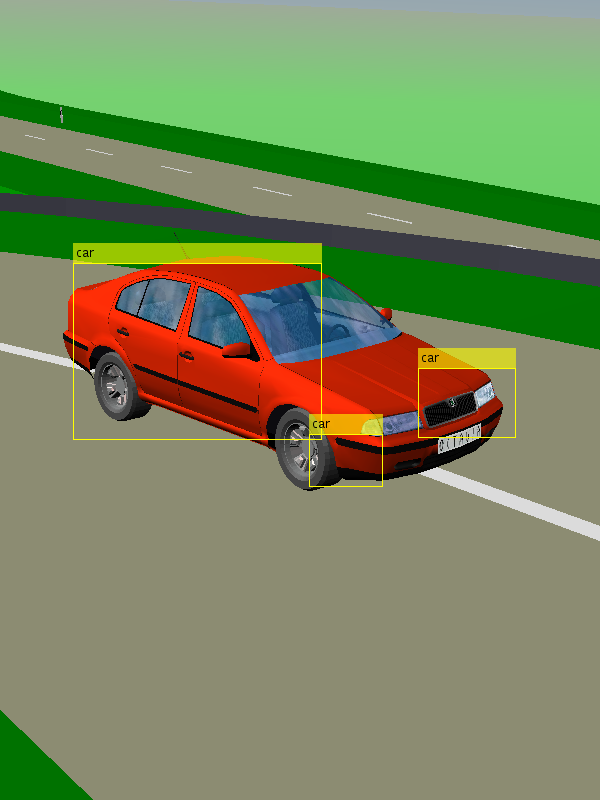
\includegraphics[scale=0.25]{figure/Haar_revelation.png}};
			
			\node (auto) at (0,0) [rectangle, minimum width=1cm, minimum height=1cm, 
			label=\textbf{HOG}] {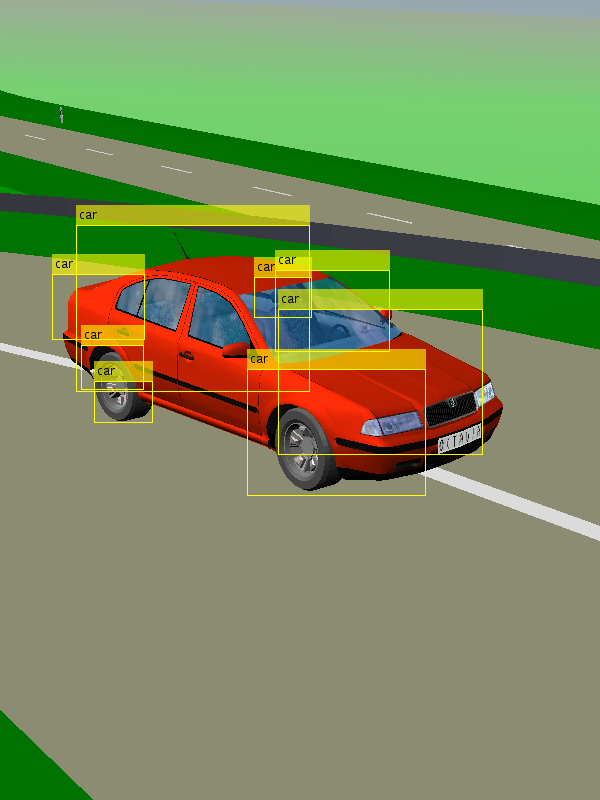
\includegraphics[scale=0.25]{figure/HOG_revelation.png}};
			
			\end{tikzpicture}
		}
	\end{center}

\end{figure}

\newpage

\section{Example \thedrawingOnImages}
\stepcounter{drawingOnImages}

\begin{figure}[h]
	\begin{center}
		\begin{tikzpicture}
		
		\draw[dashed] (0,0) coordinate -- (0,1.3) coordinate;
		\draw[->] (0,1.3) coordinate -- (0,5) coordinate node[above left]{$Y$};
		\draw[dashed] (0,0) coordinate -- (1.6,0) coordinate;
		\draw[->] (1.6,0) coordinate -- (3,0) coordinate node[above right]{$X$};
		\draw[dashed] (0,0) coordinate -- (-0.5,-0.5) coordinate;
		\draw[->] (-0.5,-0.5) coordinate -- (-2,-2) coordinate node[above left]{$Z$};
		\draw[dashed] (0,0) coordinate -- (1,1) coordinate;
		\draw[-] (1,1) coordinate -- (3,3) coordinate node[below right]{$-Z$};
		\draw[-] (-1.6,0) coordinate -- (-6,0) coordinate;
		
		\draw[dashed] (-5,-1) coordinate -- (-5,4) coordinate;
		\draw[dashed] (-4,0) coordinate -- (-5,-1) coordinate;
		\draw[dashed] (-5,-1) coordinate -- (-1,-1) coordinate;
		
		\draw[dashed] (-5,-1) coordinate (a) -- (0,0) coordinate (b) -- (-5,4) coordinate (c)
		pic["$\mathbf{\beta}$", draw, <-, angle eccentricity=1.2, angle radius=2.5cm, line width=1.25pt]{angle=c--b--a};
		
		\draw[dashed] (-4,0) coordinate (d) -- (0,0) coordinate (e);
		
		\draw[dashed] pic["$\mathbf{\alpha}$", draw, ->, angle eccentricity=1.2, angle radius=3.25cm, line width=1.25pt]{angle=d--e--a};
		
		\draw (-3,2.7) coordinate node[above]{$r$};
		
		\draw (-6,5) coordinate node[above]{$\mathbf{Camera}$};
		\draw (2,-1) coordinate node[above left]{$\mathbf{Car}$};
		
		\node at (-5,5) []{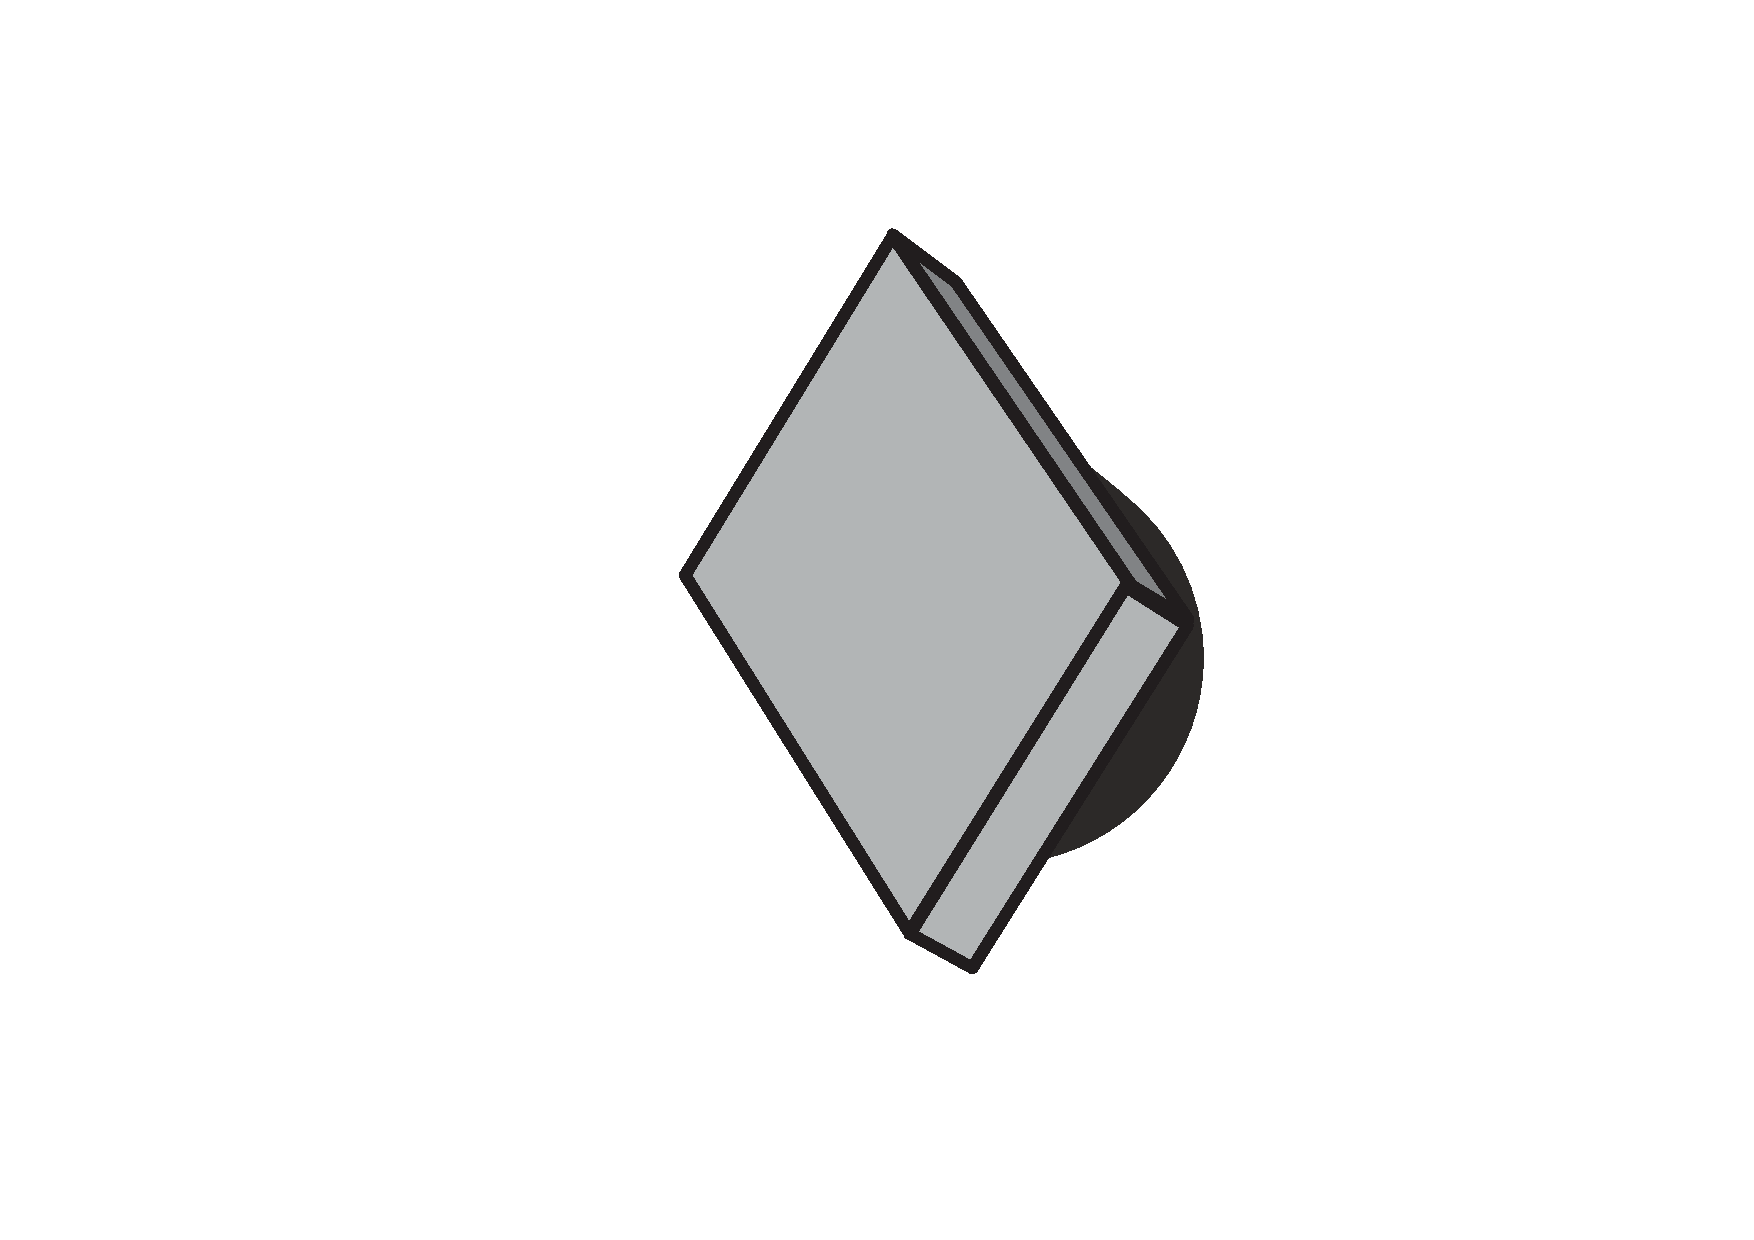
\includegraphics[scale=0.15, trim=17cm 18cm 15cm 45cm]{pdf/camera.pdf}};
		\node at (2,-1) []{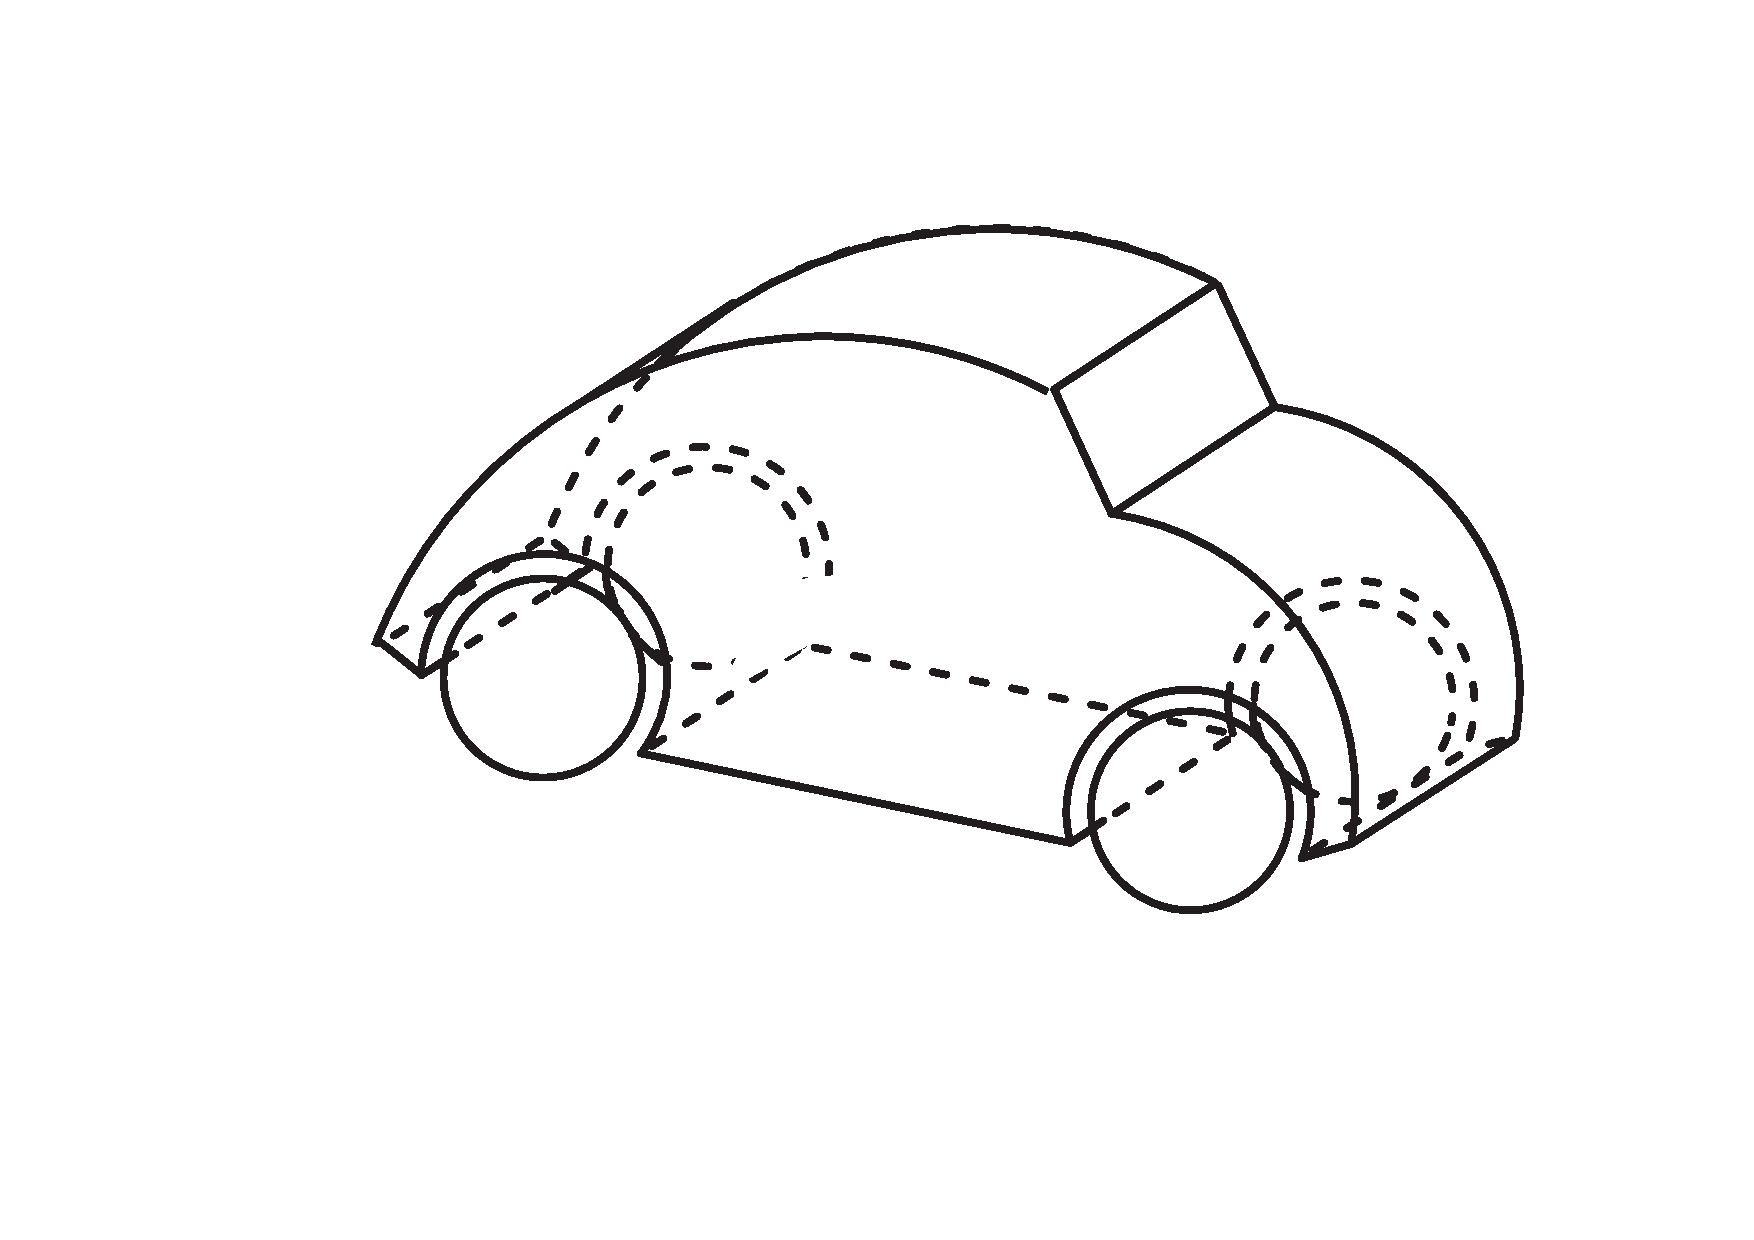
\includegraphics[scale=0.15, trim=17cm 3cm -12cm 45cm]{pdf/auto.pdf}};
		
		
		\end{tikzpicture}
	\end{center}
	
\end{figure}


\section{Example \thedrawingOnImages}
\stepcounter{drawingOnImages}

\begin{figure}[h]
	\begin{center}
		\scalebox{0.85}{
			\begin{tikzpicture}
			
			\draw[latex-] (0.15,2.3) arc (-25:-110:0.30cm) node[above left]{$\psi$};
			\draw[latex-] (-1.9,-1.085) arc (35:-150:0.30cm);
			\draw (-1.7,-1.3) node[below]{$\phi$};
			\draw[latex-] (1.8,-1.125) arc (115:-100:0.30cm) node[below right]{$\theta$};
			
			\draw[-latex] (0,0) coordinate -- (0,3) coordinate node[anchor=west]{$u_{z}$};
			\draw[-latex] (0,0) coordinate -- (-2.5,-1.625) coordinate node[below left]{$u_{x}$};
			\draw[-latex] (0,0) coordinate -- (2.5,-1.625) coordinate node[below right]{$u_{y}$};
			\draw (-0.05,0.9) node[below right]{$O_{ABC}$};
			
			\node (esacottero) at (0,-0.25) [text 
			centered]{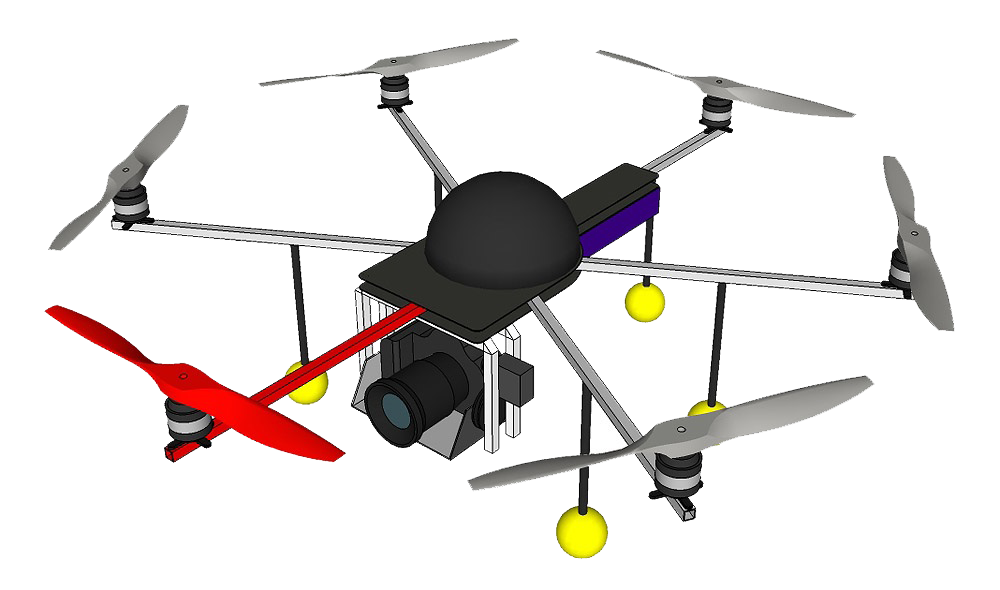
\includegraphics[scale=0.15]{figure/hexarotor_CAD_transparent.png}};
			
			\draw[latex-] (-1.475,-0.385) arc (-25:-100:0.30cm);
			\draw[-latex] (-1.78,0.7) arc (-35:-110:0.30cm);
			\draw[latex-] (-0.365,1.275) arc (-25:-100:0.30cm);
			\draw[-latex] (1.325,1.175) arc (-45:-110:0.30cm);
			\draw[latex-] (2.395,0.3725) arc (-25:-100:0.30cm);
			\draw[-latex] (1.1625,-0.5725) arc (-25:-100:0.30cm);
			
			\draw[-latex] (-1.675,-0.685) coordinate -- (-1.675,-0.185) node[left]{$\Omega_1$};
			\draw[-latex] (-1.98,0.4) coordinate -- (-1.98,0.9) node[left]{$\Omega_6$};
			\draw[-latex] (-0.565,0.975) coordinate -- (-0.565,1.475) node[left]{$\Omega_5$};
			\draw[-latex] (1.165,0.875) coordinate -- (1.165,1.375) node[left]{$\Omega_4$};
			\draw[-latex] (2.195,0.0725) coordinate -- (2.195,0.5725) node[right]{$\Omega_3$};
			\draw[-latex] (0.9625,-0.9725) coordinate -- (0.9625,-0.4725) coordinate;
			\draw (1.4625,-0.7725) node[above]{$\Omega_2$};
			
			\draw[latex-] (-4.3,-1.5) arc (-25:-110:0.30cm) node[left]{$\psi$};
			\draw[latex-] (-3.15,-4) arc (55:-110:0.30cm) node[below right]{$\theta$};
			\draw[latex-] (-6.1,-3.8) arc (115:-100:0.30cm) node[below right]{$\phi$};
			
			\draw[-latex] (-4.5,-3) coordinate -- (-4.5,0) coordinate node[anchor=east]{$u_{z}$};
			\draw[-latex] (-4.5,-3) coordinate -- (-7,-5) coordinate node[below right]{$u_{x}$};
			\draw[-latex] (-4.5,-3) coordinate -- (-2.5,-5) coordinate node[below left]{$u_{y}$};
			\draw (-4.5,-3) node[right]{$O_{FI}$};
			
			\end{tikzpicture}
		}
	\end{center}
	
\end{figure}

\newpage

\section{Example \thedrawingOnImages}
\stepcounter{drawingOnImages}

\begin{figure}[h]
	\begin{center}
		\scalebox{0.95}{
			\begin{tikzpicture}[node distance=2cm]
					
			\node (classifier) at (0,0) [rectangle, draw, text centered, minimum width=2.5cm, 
			minimum height=1cm] {Classifier};
			
			\node (faceDetectionSystem) at (0,-4) [rectangle, draw, text centered, minimum 
			width=2.5cm, minimum height=1cm] {Faces recognition};
			
			\node (endrix) at (-5,-4) [rectangle, minimum width=1cm, minimum height=1cm] {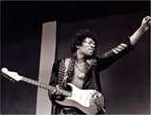
\includegraphics[scale=0.8]{figure/endrix.png}};
			
			\node (endrixKnown) at (5,-4) [rectangle, minimum width=2cm, minimum height=1cm] 
			{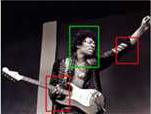
\includegraphics[scale=0.8]{figure/endrixKnown.png}};
			
			\node (truePositive) at (5,1) [rectangle, minimum width=2cm, minimum height=1cm, 
			label=False positive] {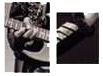
\includegraphics[scale=1]{figure/truePositivePhoto.png}};
			
			\node (dataSet) at (-5,1) [rectangle, minimum width=2cm, minimum height=1cm, 
			label=Initial Dataset] {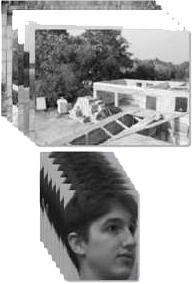
\includegraphics[scale=0.6]{figure/dataSet.png}};
			
			\draw [-latex] (classifier.south) -- (faceDetectionSystem.north);
			
			\draw [-latex] (endrix.east) -- (faceDetectionSystem.west);
			
			\draw [-latex] (endrixKnown.north) -- (truePositive.south);
			
			\draw [-latex] (faceDetectionSystem.east) -- (endrixKnown.west);
			
			\draw [-latex] (dataSet) to [out=0,in=90] (classifier);
			\draw [-latex] (truePositive) to [out=180,in=90] (classifier);
			
			\end{tikzpicture}
		}
	\end{center}
\end{figure}

\section{Example \thedrawingOnImages}
\stepcounter{drawingOnImages}

\begin{figure}[h]
	\begin{center}
		\scalebox{0.8}{
		\begin{tikzpicture}
		
		\draw[-latex] (0,0) coordinate -- (0,3) coordinate node[above right]{$Y_w$};
		\draw[-latex] (0,0) coordinate -- (3,0) coordinate node[above right]{$X_w$};
		
		\draw[-latex] (5.2,5.2) coordinate -- (7,7) coordinate node[above right]{$X_b$};
		\draw[-latex] (5.2,5.2) coordinate -- (5.2,7.5) coordinate;
		
		\draw (5.2,7.5) coordinate (a) -- (5.2,5.2) coordinate (b) -- (7,7) coordinate (c)
		pic["$\mathbf{\psi}$", draw, latex-, angle eccentricity=1.2, angle radius=1.5cm]{angle=c--b--a};
		
		\node (drone) at (4,4) [text centered]{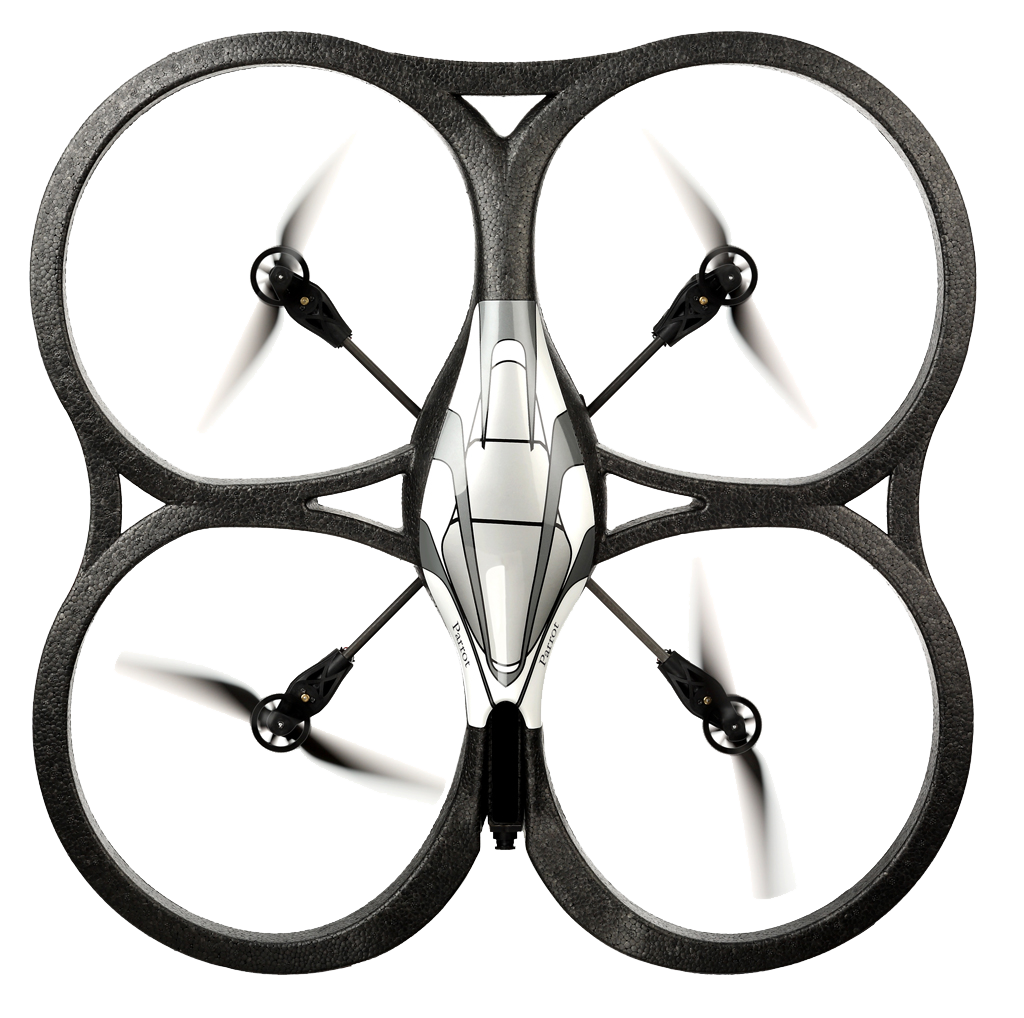
\includegraphics[scale=0.5, angle=-225]{figure/ARDrone_front.png}};
		
		\end{tikzpicture}
	}
	\end{center}
	
\end{figure}

\newpage

\section{Example \thedrawingOnImages}
\stepcounter{drawingOnImages}

	\begin{figure}[h]
	\begin{center}
		\scalebox{0.85}{			
			\begin{tikzpicture}
			\node (stazioneTerra) at (-4,0) 
			{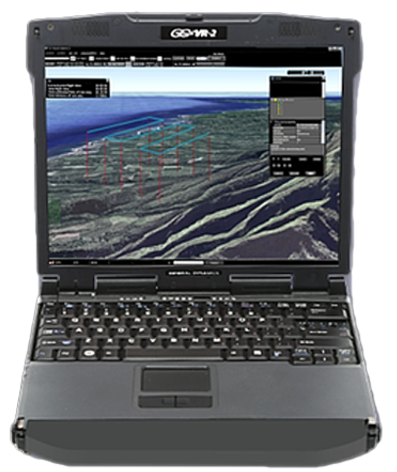
\includegraphics[scale=0.25]{figure/groundStation.png}};
			\node (drone) at (2.5,0) {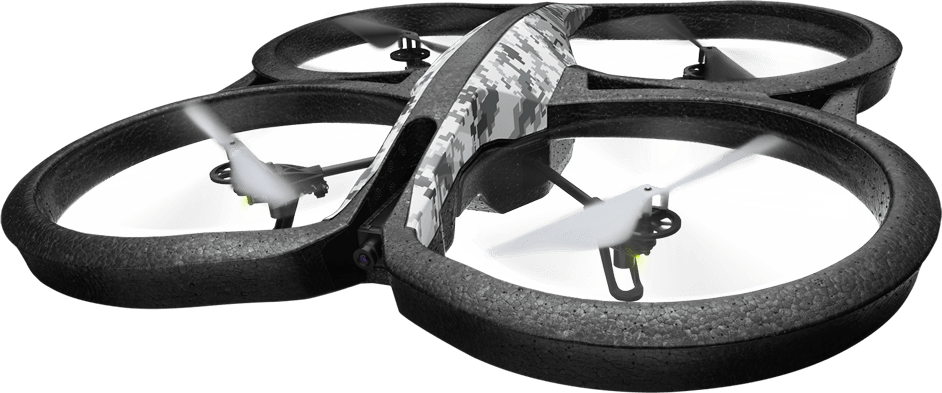
\includegraphics[scale=0.2]{figure/droneSnow.png}};
			\node (drone) at (-0.5,2.8) {
\includegraphics[scale=0.2]{figure/redArrow.png}};
			\node (drone) at (-0.5,-2.8) {
\includegraphics[scale=0.2]{figure/bluArrow.png}};	
			\end{tikzpicture}	
		}
	\end{center}
\end{figure}


\section{Example \thedrawingOnImages}
\stepcounter{drawingOnImages}

\begin{figure}[h]
	\begin{center}
		\scalebox{0.9}{
		\begin{tikzpicture}
		\node (graphic) at (0,0) [text 
		centered]{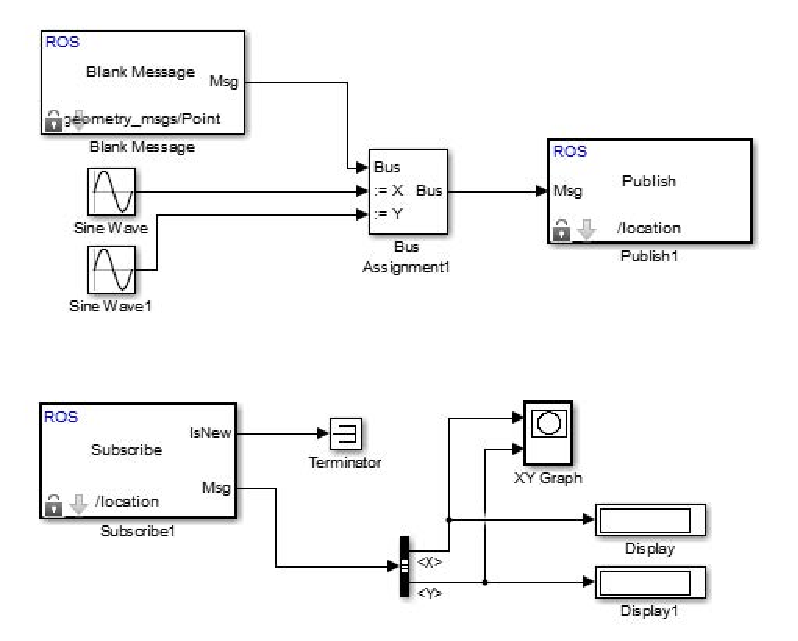
\includegraphics[scale=0.85]{pdf/intro_subsub_msgs}};
		
		\node (frame1) at (0,2.15) [draw, rectangle, dashed, text centered, red!75, minimum 
		height=4.75cm, minimum width=12cm, line width=2.5pt]{};
		
		\node (frame2) at (0,-2.75) [draw, rectangle, dashed, text centered, green!75, minimum 
		height=4cm, minimum width=12cm, line width=2.5pt]{};
		\end{tikzpicture}
	}
	\end{center}

\end{figure}

\newpage

\section{Example \thedrawingOnImages}
\stepcounter{drawingOnImages}

\begin{figure}[h]
	\begin{center}
			\begin{tikzpicture}
			
			\draw[latex-] (0.25,2.3) arc (-25:-110:0.30cm) node[above left]{$\psi$};
			\draw[latex-] (-1.0,-0.9) arc (45:-110:0.30cm);
			\draw (-1.0,-0.9) node[below right]{$\phi$};
			\draw[latex-] (1.825,-0.2) arc (105:-70:0.30cm);
			\draw (2.05,-0.25) node[right]{$\theta$};
			
			\draw[-latex] (0.05,0) coordinate -- (0.05,3) coordinate node[anchor=west]{$e_{z}$};
			\draw[-latex] (0.05,0) coordinate -- (-1.60,-1.55) coordinate node[left]{$e_{x}$};
			\draw[-latex] (0.05,-0.1) coordinate -- (2.55,-0.6) coordinate node[below right]{$e_{y}$};
			\draw (0.05,0.8) node[below right]{$O_{ABC}$};
			
			\node (esacottero) at (0,0) [text centered]{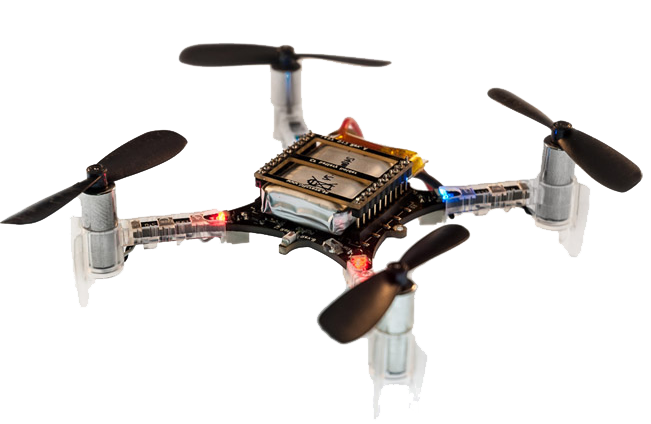
\includegraphics[scale=0.2]{figure/Crazyflie20_1.png}};
			
			\draw[-latex] (-1.3,0.655) arc (55:-15:0.35cm); %omega 1
			\draw[latex-] (-0.05,1.225) arc (-25:-120:0.30cm); %omega 2
			\draw[-latex] (1.2,0.87) arc (55:-15:0.35cm); %omega 3
			\draw[latex-] (0.6225,0.125) arc (-25:-120:0.30cm); %omega 4
			
			\draw[-latex] (-1.225,0.3) coordinate -- (-1.225,0.9) node[left]{$\omega_1$};
			\draw[-latex] (-0.21,0.9) coordinate -- (-0.21,1.5) node[left]{$\omega_2$};
			\draw[-latex] (1.26,0.525) coordinate -- (1.26,1.125) node[right]{$\omega_3$};
			\draw[-latex] (0.36,-0.25) coordinate -- (0.36,0.35) coordinate;
			\draw (0.85,-0.7225) node[above]{$\omega_4$};
			
			\draw[latex-] (-2.9,-2.5) arc (-25:-110:0.30cm) node[left]{$\psi$};
			\draw[latex-] (-2.475,-5.9) arc (105:-70:0.30cm);
			\draw (-2.15,-6.15) node[right]{$\theta$};
			\draw[latex-] (-5.4,-4.9) arc (45:-130:0.30cm);
			\draw (-5.6,-5.3) node[below right]{$\phi$};
			
			\draw[-latex] (-3.05,-5) coordinate -- (-3.05,-2) coordinate node[anchor=east]{$e_{z}$};
			\draw[-latex] (-3.05,-5) coordinate -- (-6.05,-5.275) coordinate node[above right]{$e_{x}$};
			\draw[-latex] (-3.05,-5) coordinate -- (-2.25,-6.725) coordinate node[below left]{$e_{y}$};
			\draw (-3.05,-5) node[right]{$O_{FI}$};
			
			\end{tikzpicture}
	\end{center}
\end{figure} 

\newpage

\section{Example \thedrawingOnImages}
\stepcounter{drawingOnImages}

\begin{figure}[h]
	\begin{center}
		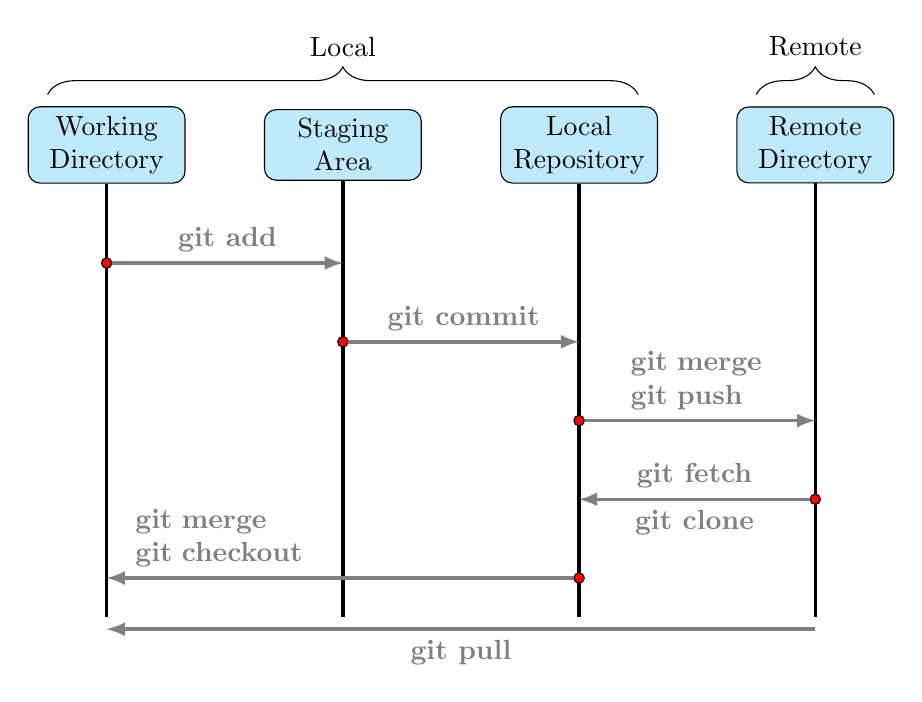
\begin{tikzpicture}
		
		\node(WorkingDirectory) at (0,0) [rounded corners=0.15cm, draw, minimum width=1.5cm, minimum height=0.75cm, rectangle, text centered, fill=cyan!25, text width=5em]{Working\\Directory};
		\node(StagingArea) at (3,0) [rounded corners=0.15cm, draw, minimum width=1.5cm, minimum height=0.75cm, rectangle, text centered, fill=cyan!25, text width=5em]{Staging\\Area};
		\node(LocalRepository) at (6,0) [rounded corners=0.15cm, draw, minimum width=1.5cm, minimum height=0.75cm, rectangle, text centered, fill=cyan!25, text width=5em]{Local\\Repository};
		\node(RemoteDirectory) at (9,0) [rounded corners=0.15cm, draw, minimum width=1.5cm, minimum height=0.75cm, rectangle, text centered, fill=cyan!25, text width=5em]{Remote\\Directory};
		
		\draw[-, line width=1.25pt] (WorkingDirectory.south) -- (0,-6);
		\draw[-, line width=1.25pt] (StagingArea.south) -- (3,-6);
		\draw[-, line width=1.25pt] (LocalRepository.south) -- (6,-6);
		\draw[-, line width=1.25pt] (RemoteDirectory.south) -- (9,-6);
		
		\node (bubble1) at (0,-1.5) [circle, draw, scale=0.4, fill=red]{};
		\node (bubble2) at (3,-2.5) [circle, draw, scale=0.4, fill=red]{};
		\node (bubble3) at (6,-3.5) [circle, draw, scale=0.4, fill=red]{};
		\node (bubble4) at (9,-4.5) [circle, draw, scale=0.4, fill=red]{};
		\node (bubble5) at (6,-5.5) [circle, draw, scale=0.4, fill=red]{};

		\draw[-latex, gray, line width=1.25pt] (bubble1) -- node[above]{\textbf{git add}} (3,-1.5) coordinate;
		\draw[-latex, gray, line width=1.25pt] (bubble2) -- node[above]{\textbf{git commit}} (6,-2.5) coordinate;
		\draw[-latex, gray, line width=1.25pt] (bubble3) -- node[above, text width=5em]{\textbf{git merge\\git push}} (9,-3.5) coordinate;
		\draw[-latex, gray, line width=1.25pt] (bubble4) -- node[above]{\textbf{git fetch}} node[below]{\textbf{git clone}} (6,-4.5) coordinate;
		\draw[-latex, gray, line width=1.25pt] (bubble5) -- node[above left, text width=7em]{\textbf{git merge\\git checkout}} (0,-5.5) coordinate;
		\draw[-latex, gray, line width=1.25pt] (9,-6.15) coordinate -- node[below]{\textbf{git pull}} (0,-6.15) coordinate;
		
		\draw [decorate,decoration={brace, amplitude=10pt,raise=4pt},yshift=0pt] (-0.75,0.5) -- (6.75,0.5) node [black,midway,xshift=0.0cm,yshift=0.75cm] {Local};
		\draw [decorate,decoration={brace, amplitude=10pt,raise=4pt},yshift=0pt] (8.25,0.5) -- (9.75,0.5) node [black,midway,xshift=0.0cm,yshift=0.75cm] {Remote};
		
		\end{tikzpicture}
	\end{center}
\end{figure}
